\documentclass[12pt]{beamer}

\usepackage{amsmath,amssymb}
\usepackage{graphicx,float}
\usepackage{minted}

\usetheme{AnnArbor}

\title[Ping Pong Bot]{Autonomous Ping Pong Collection Robot}
\subtitle[EECS 373 Project]{EECS 373, Intro. to Embedded System Design Project}
\author[Qin, Chen, Wan, Gao]{Binhao Qin, Che Chen, Hanxi Wan, Yijia Gao}
\date{\today}
	
\AtBeginSection[]
{
    \begin{frame}
        \frametitle{Table of Contents}
        \tableofcontents[currentsection]
    \end{frame}
}

\AtEndDocument{
    \begin{frame}
        \centering
        \LARGE
        Thank you!\\
        Q \& A
    \end{frame}
}

\begin{document}
\frame{\titlepage}
\begin{frame}
    \frametitle{Table of Contents}
    \tableofcontents
\end{frame}

\section{Introduction}
\begin{frame}
    \frametitle{Overview}
    \begin{itemize}
        \item Table Tennis Multi-ball Training
        \item Collecting balls is tiring and time-wasting
        \item Avoid body pain caused by frequently bending down
    \end{itemize}
    \begin{figure}
        \centering
        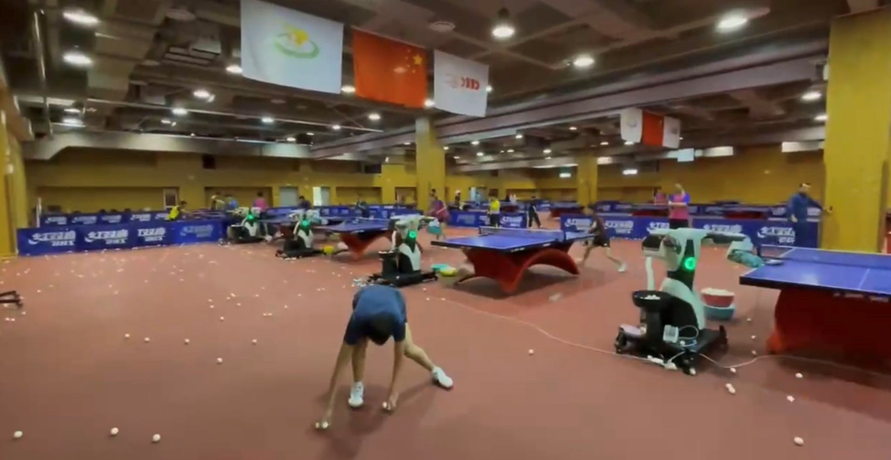
\includegraphics[width=0.7\textwidth]{Picture/tableTennisPic.png}
    \end{figure}
\end{frame}

\begin{frame}{Main Features}
    \begin{itemize}
        \item Collector: 1 servo, 3D printed components
        \item Motion: 4 mecanum wheels, motors (H-Bridge, PWM)
        \item CV: recognition \& localization
        \item Inter-Controller UART Communication
        \item Manual mode: debugging and playing with N64 Controller
        \item Displaying statistics: LCD, I2C
    \end{itemize}
\end{frame}

\section{Mechanical Parts and Locomotion}

\begin{frame}
    \frametitle{Collector Design}
    \begin{itemize}
        \item roller with rubber bands to ``catch'' and reserve balls
        \item motor free, rolled by friction
        \item servo to add pressure or raise the roller up
    \end{itemize}
    \begin{figure}[H]
        \centering
        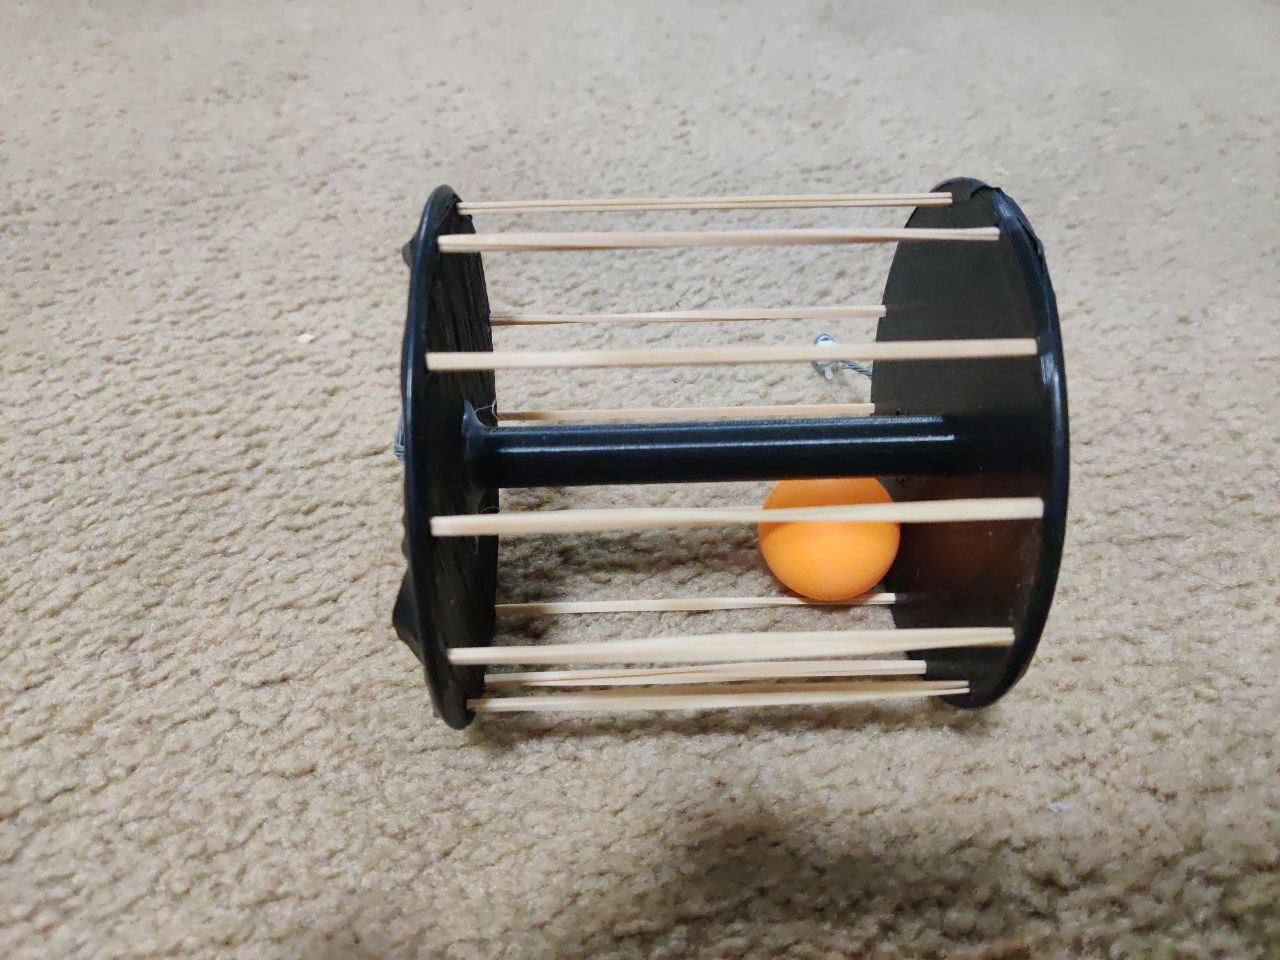
\includegraphics[width=0.5\textwidth]{Picture/collector.jpg}
        \caption{Roller with a ball}
    \end{figure}
\end{frame}

\begin{frame}{Motors and Servos}
    \begin{columns}
        \begin{column}{.65\linewidth}
            \begin{itemize}
                \item Task
                      \begin{itemize}
                          \item Control totally 4 motors and 1 servo
                      \end{itemize}
                \item Solution
                      \begin{itemize}
                          \item Motor Shield
                                \begin{itemize}
                                    \item 1 * PCA9685 I2C PWM Controller
                                    \item 2 * TB6612 DC drivers
                                \end{itemize}
                          \item Send command via I2C to set PWM Controller, which controls motor drivers and servos
                      \end{itemize}

            \end{itemize}
        \end{column}
        \begin{column}{.3\linewidth}
            \begin{figure}[H]
                \centering
                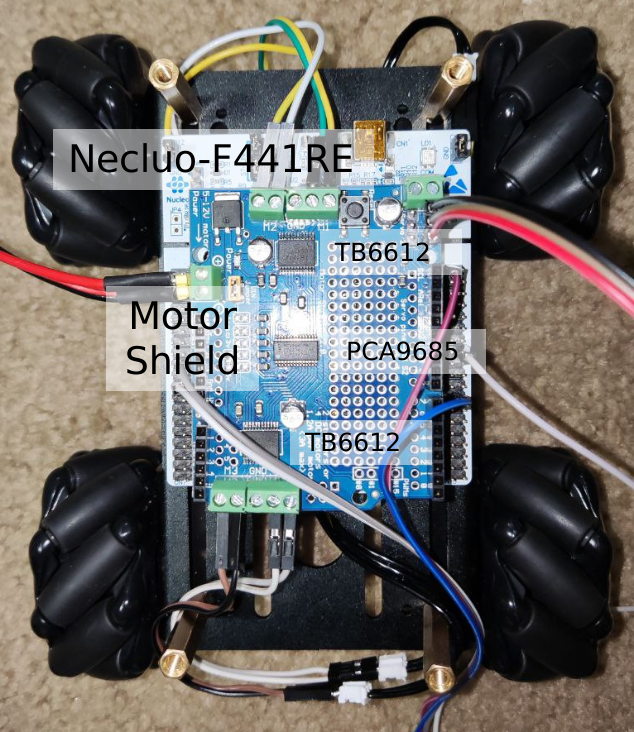
\includegraphics[width=\textwidth]{motorshield.png}
            \end{figure}
        \end{column}
    \end{columns}

\end{frame}

\begin{frame}{Motors and Servos}
    \begin{columns}
        \begin{column}{.65\linewidth}
            \begin{itemize}
                \item Challenge
                      \begin{itemize}
                          \item Datasheets available for PWM Controller and DC drivers, but\\
                                no datasheet for the Motor Shield
                      \end{itemize}
                \item Solution
                      \begin{itemize}
                          \item Refer to Arduino library provided by MotorShield manufacturer
                          \item Use logic analyzer to debug I2C transmission
                      \end{itemize}

            \end{itemize}
        \end{column}
        \begin{column}{.3\linewidth}
            \begin{figure}[H]
                \centering
                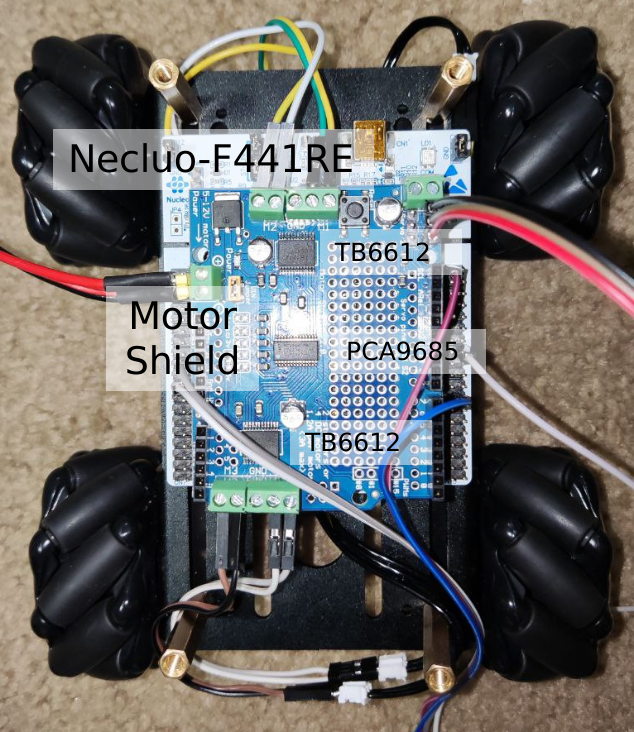
\includegraphics[width=\textwidth]{motorshield.png}
            \end{figure}
        \end{column}
    \end{columns}
\end{frame}

\section{Computer Vision: Recognition \& Localization}
\begin{frame}
    \frametitle{Ball Recognition}
    \begin{itemize}
        \item assume ping-pong ball to be yellow
        \item convert to HSV color space for easy color extraction
        \item extract a range of color from the frame that may be the ball
        \item find contours on the extracted mask
        \item for big contours, calculate the mininum enclosing circle to be the ball
    \end{itemize}
\end{frame}

\begin{frame}
    \frametitle{Localization}
    \begin{itemize}
        \item We know the actual radius of the ball $R$, focal length $f$, and size of the ball on the frame $r$
        \item The distance of the ball $d$ can be calculated as $d = \frac{fR}{r}$
        \item Thus the position of the ball in camera coordinate can be calculated
        \item Match the balls with previous frame using ICP algorithm and get the camera motion
    \end{itemize}
    \begin{figure}[H]
        \centering
        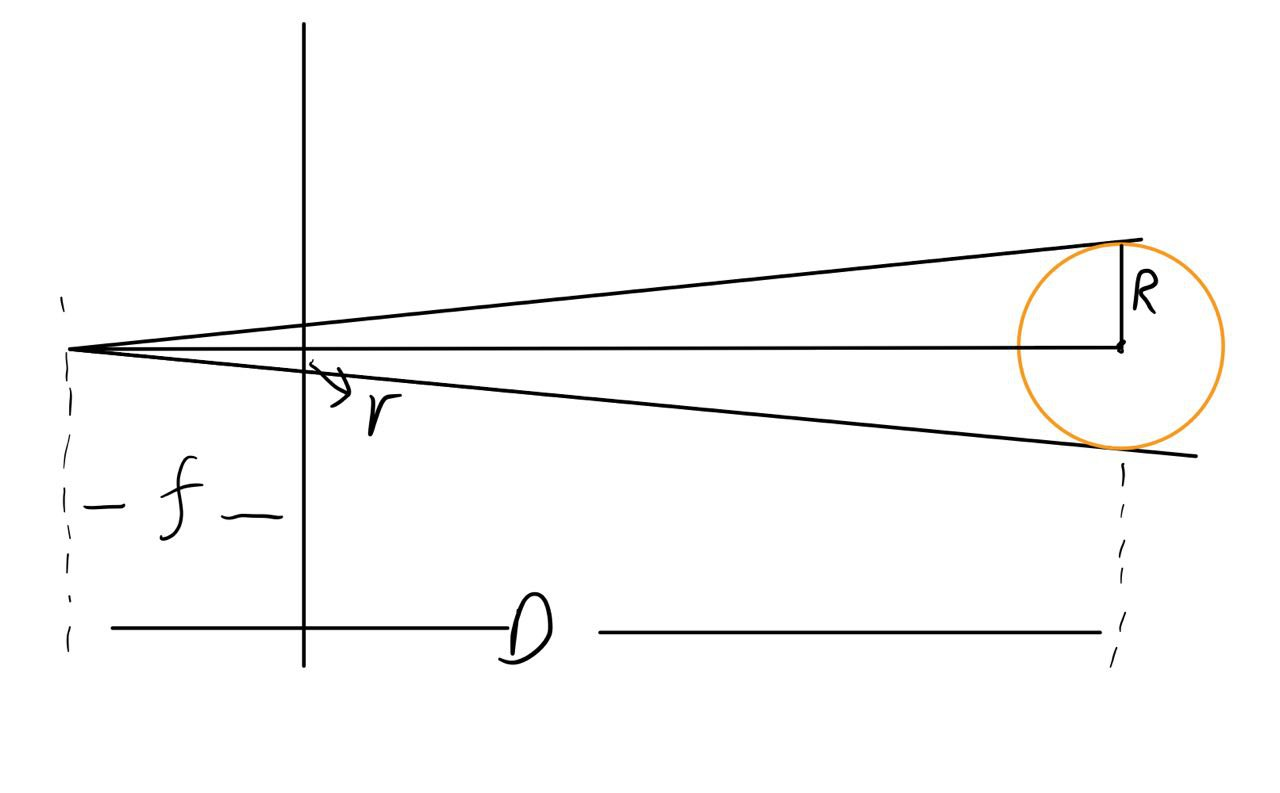
\includegraphics[width=0.4\textwidth]{Picture/ball_distance.jpg}
    \end{figure}
\end{frame}

\section{Inter-Controller Communication}
\begin{frame}
    \frametitle{Inter-Controller Communication}
    \begin{itemize}
        \item Recognition and Localization computed on Raspberry Pi, need to give control information to STM32 board
        \item Serial UART communication is used
        \item Task: defining an efficient and stable communication protocol
        \item Solution:
              \begin{itemize}
                  \item 2 0xFF to start transaction
                  \item 1 Header byte to indicate device to operate
                  \item 1 or 2 data byte(s) depending on device type
                  \item 2 0xFF to end transaction
                  \item slave device transmit 1 byte to ensure completion
              \end{itemize}
    \end{itemize}
\end{frame}

\section{Interfacing N64 Controller}
\begin{frame}
    \frametitle{N64 Controller Protocol}
    \begin{itemize}
        \item 1-wire, half-duplex serial protocol
        \item OD/OC circuit with pull-up resistor required to avoid multi-driver issue
        \item 3-4 $\mu$s per bit transaction, and at least 2x sampling rate for receiver, which is sub-megahertz
        \item little endian but MSB first instead of LSB first
    \end{itemize}
    \begin{figure}[H]
        \centering
        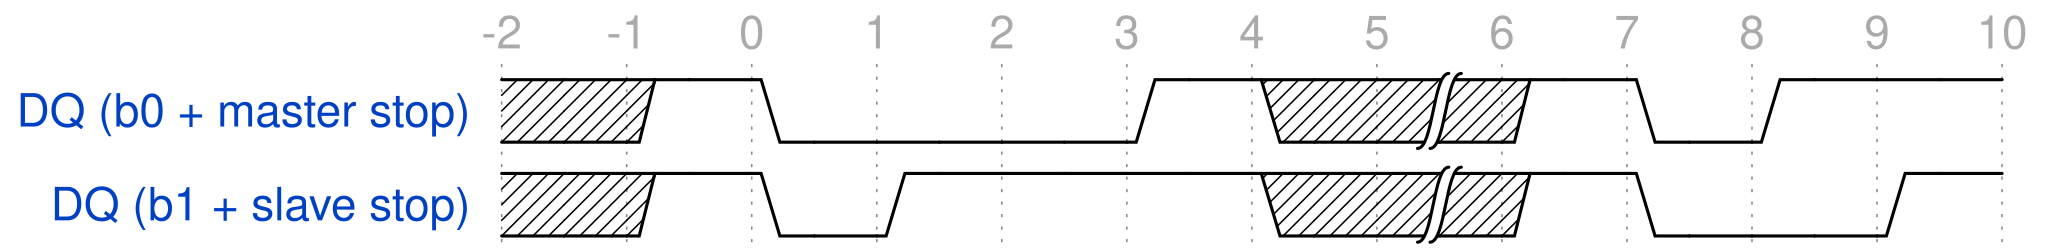
\includegraphics[width=0.9\textwidth]{N64_drom.png}
        \caption{Timing Diagram of Bit Transaction}
    \end{figure}
    \begin{itemize}
        \item \textbf{What is the major difficulty in implementation?}
    \end{itemize}
\end{frame}

\begin{frame}
    \frametitle{Interfacing Challenges}
    \begin{itemize}
        \item Welcome to real-time programming!
        \item \textbf{Time is precious resource!!!}
              \begin{itemize}
                  \item OD/OC design makes rising edge slow
                  \item internal pull-up resistor with 40k$\Omega$ is catastrophic
                  \item need microsecond level delay, but timer MMIO is slow
                  \item interrupts/buffering cannot be tolerated
                  \item memory accesses cannot be tolerated
                  \item function calls with stack pushes/branching cannot be tolerated
              \end{itemize}
        \item Solutions:
              \begin{itemize}
                  \item use small external pull-up resistor (4.7k$\Omega$)
                  \item implement microsecond delay by counting instructions
                  \item RAII CPU mutex locks interrupts for atomicity
                  \item use very few variables inside critical section
                  \item force function calls to be inline inside critical section
              \end{itemize}
    \end{itemize}
\end{frame}

\begin{frame}[fragile]
    \frametitle{A New Issue: Mix Compiling C/C++}
    \begin{itemize}
        \item As stated before, in order to meet the timing requirements, we would like to have RAII mutexes and inline functions.
        \item This cannot be easily achieved using C, and therefore C++ is used to implement these features.
        \item \textbf{However, C/C++ name function labels differently in assembly:}
              \begin{itemize}
                  \item C: \verb|int f(int);| compiles to \verb|f:|
                  \item C++: \verb|int f(int);| compiles to \verb|_Z1fi:|
                  \item Need \verb|extern "C"| syntax to tell the compiler about C functions
              \end{itemize}
        \item More on this topic: Check out name mangling on the Internet
    \end{itemize}
\end{frame}

\section{Setting Up LCD}
\begin{frame}[fragile]
    \frametitle{Setting Up LCD}
    \begin{itemize}
        \item Challenges: sending 8-bit data/command through 4-bit channel
        \item Solutions:
              \begin{itemize}
                  \item EN falling edge sensitive, 2 transactions per byte
                  \item Cut the data in Upper 4-bit and Lower 4-bit
                  \item Configure data and send
              \end{itemize}
    \end{itemize}
    \scriptsize
    \begin{minted}{cpp}
    void LCD::send(uint8_t byte, bool type)
    {
	    uint8_t encoded[4] = {0};
	    uint8_t byteHigh = byte & 0xF0;
	    uint8_t byteLow = (byte & 0x0F) << 4;
	    encoded[0] = byteHigh | enableHigh | (type & 0b1);
	    encoded[1] = byteHigh | enableLow | (type & 0b1);
	    encoded[2] = byteLow | enableHigh | (type & 0b1);
	    encoded[3] = byteLow | enableLow | (type & 0b1);
	    HAL_I2C_Master_Transmit(&i2c, address, encoded, 4, HAL_MAX_DELAY);
    }
    \end{minted}
\end{frame}

\section{Next Step}
\begin{frame}{Next Step}
    \begin{itemize}
        \item Assembly all the parts
        \item Set up simulation environment
        \item Conduct all-around testing
    \end{itemize}
\end{frame}

\section*{}

\end{document}
